\section{ViT vs. CNN}

\begin{frame}{Inductive Bias}
    \begin{itemize}
        \item In CNNs, locality, 2D neighborhood structure, and translation equivariance are baked into each layer throughout the whole model.
        \item In ViT, only MLP layers exhibit locality and translational equivariance, while self-attention layers capture global context.
        \item The 2D neighborhood structure is used very sparingly.
    \end{itemize}
\end{frame}

\begin{frame}{Combining CNNs and Transformers}
    \begin{itemize}
        \item As an alternative to raw image patches, the input sequence can be formed from feature maps of a CNN.
	    \item These hybrid models combine the local feature extraction capabilities of CNNs with the global context awareness of Transformers. 
        \item These models can perform well even on smaller datasets.
    \end{itemize}
\end{frame}

\begin{frame}{Dataset Size}
    \begin{columns}
        \begin{column}{0.5\textwidth}
            \begin{figure}
                \centering
                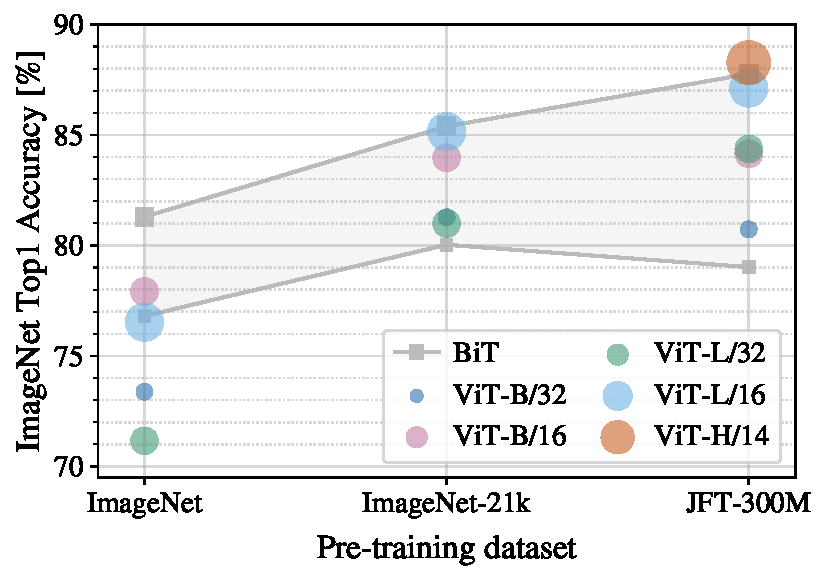
\includegraphics[width=\textwidth]{pic/transvolution-i1k-scaling}
                % \caption{
                % % Transfer to ImageNet. 
                % While large ViT models perform worse than BiT ResNets when pre-trained on small datasets, they shine when pre-trained on larger datasets. 
                % %Similarly, larger ViT variants overtake smaller ones as the dataset grows.
                % }
                \label{fig:transvolution}
            \end{figure}
        \end{column}
        \begin{column}{0.5\textwidth}
            \begin{figure}
                \centering
                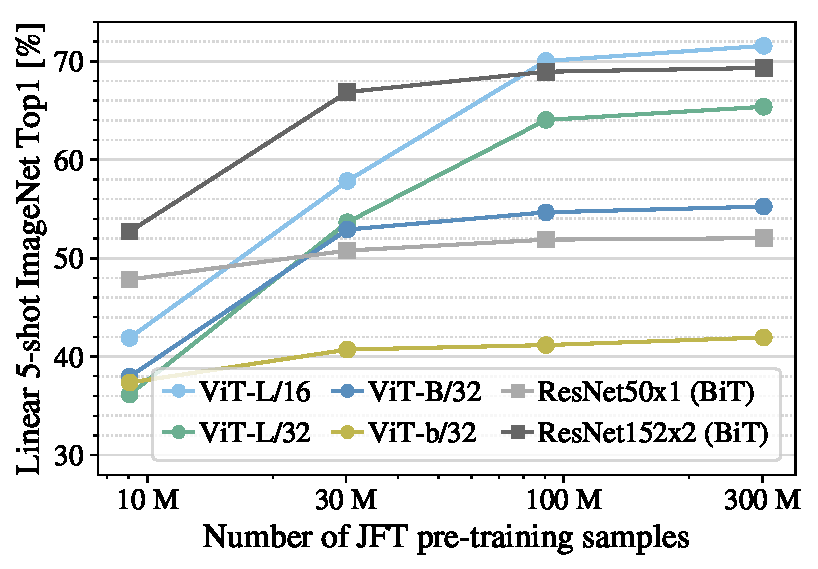
\includegraphics[width=\textwidth]{pic/imagenet_5shot}
                % \caption{
                % % Linear few-shot evaluation on ImageNet versus pre-training size. 
                % ResNets perform better with smaller pre-training datasets but plateau sooner than ViT, which performs better with larger pre-training. 
                % %ViT-b is ViT-B with all hidden dimensions halved.
                % }
                \label{fig:imagenet_5shot}
            \end{figure}
        \end{column}
    \end{columns}
\end{frame}


\begin{frame}{Performance vs. Pre-training}
    \begin{figure}
        \centering
        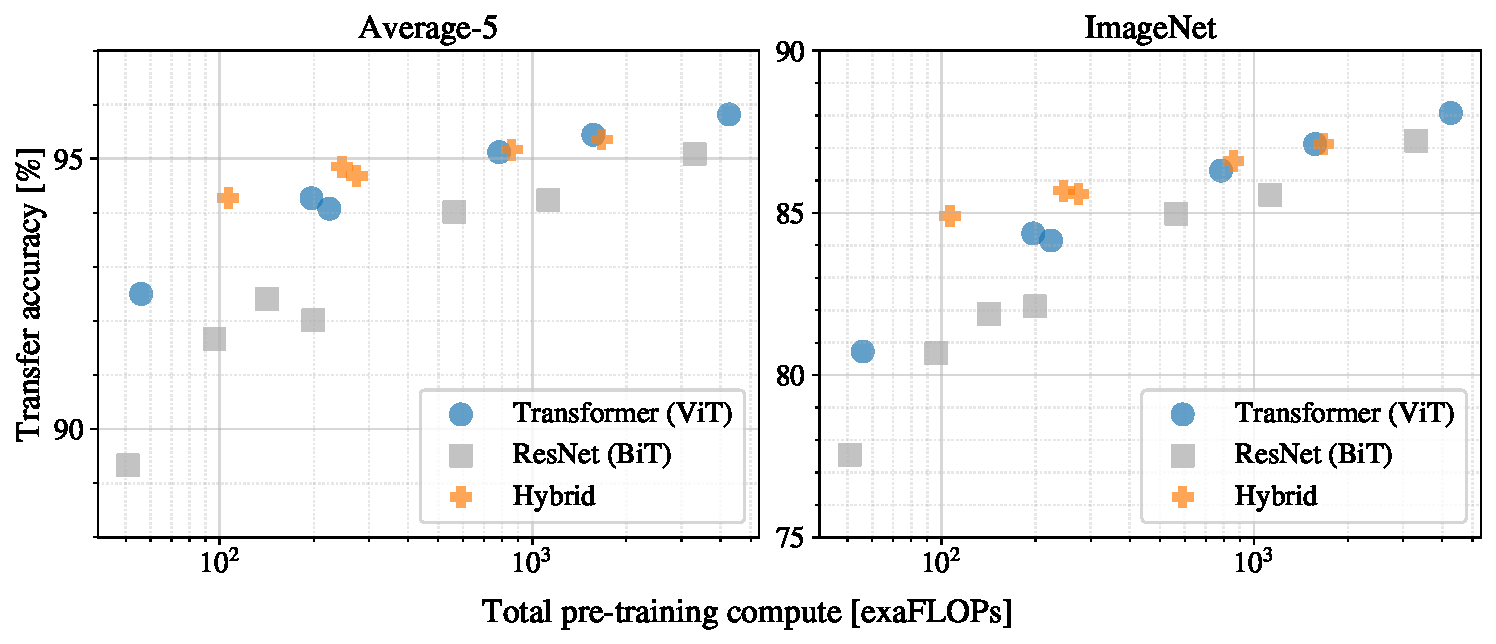
\includegraphics[width=0.9\linewidth]{pic/finetune_vs_compute2.pdf}
        % \caption{Vision Transformers generally outperform ResNets with the same computational budget. Hybrids improve upon pure Transformers for smaller model sizes, but the gap vanishes for larger models.}
        \label{fig:enter-label}
    \end{figure}
\end{frame}


\begin{frame}{State-of-the-Art}
    \begin{itemize}
        \item Transformers achieve State-of-the-Art results in a variety of computer vision tasks, including \textbf{Classification}, \textbf{Segmentation}, \textbf{Detection}, and more!
    \end{itemize}
    \begin{figure}
        \centering
        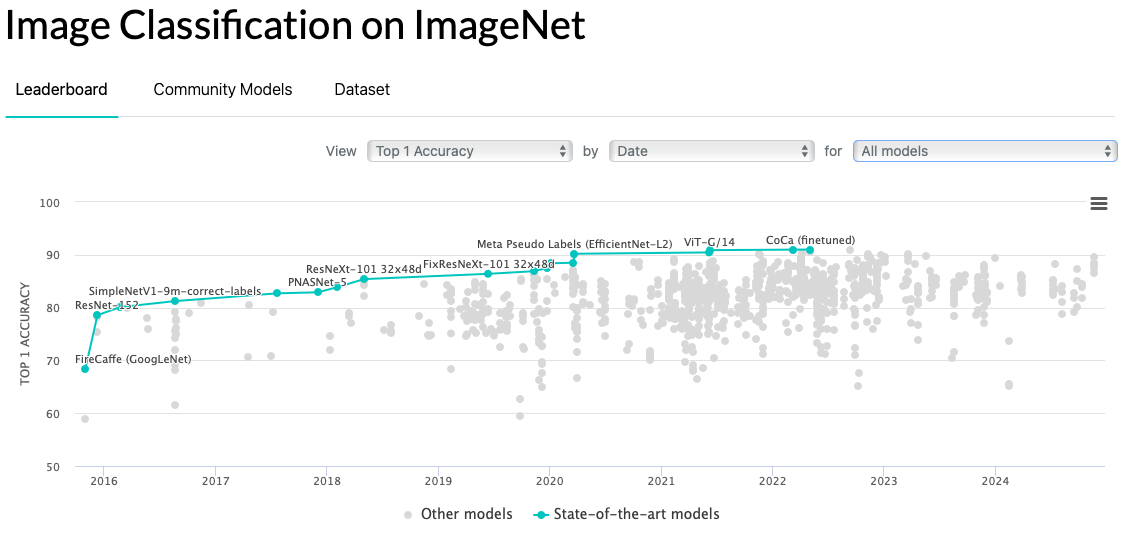
\includegraphics[width=\linewidth]{pic/SOTA.png}
        % \caption{State-of-the-Art Performance}
        \label{fig:sota}
    \end{figure}
\end{frame}

\begin{frame}{Conclusion}
    \begin{itemize}
        \item \textbf{Advantages of ViTs}
        \begin{itemize}
            \item \textbf{Better with Scale}: Performance improves significantly as dataset size and model size grow.
            \item \textbf{Unified Architecture}: The same Transformer blocks can be applied to text, images, and other modalities.
            \item \textbf{Interpretability}: Attention maps can provide insights into which patches are influencing the final decision.
        \end{itemize}
        \item \textbf{Disadvantages of ViTs}
        \begin{itemize}
            \item \textbf{Data Hungry}: ViTs typically require large pretraining datasets.
            \item \textbf{Computational Cost}: Multi-head self-attention scales quadratically with the number of tokens. For high-resolution images, this can be expensive.
            \item \textbf{Overfitting}: High capacity can lead to overfitting.
        \end{itemize}
    \end{itemize}
\end{frame}

